\chapter{Background}

\quad Parallel computing and software parallelization are the vast overlapping and complementary computer science areas with a history dating back to 1950s. With the advances in semiconductor industry the topics have left from high-end scientific supercomputers niche and spread to a much wider area spanning to all consumer electronic devices and are of major importance now. The parallelism is pervasive and all. Every computer scientist, software developer would benefit from having an insight into the area. Nonetheless the topics are extremely difficult and require a great deal of knowledge in various subtopics. Not all 

\section{The importance of parallel computing}
\label{parallel_computing_importance}
\quad The parallelism is pervasive and the future of computing is parallel. There are numerous factors which stress the importance of parallelism in modern computing.   

\begin{description}
\item[Abundance of natural parallelism] The field of High Performance Computing (HPC) has traditionally been concerned with scientific modelling and simulation of various natural phenomena (climate change, fluid flows, etc.). Such systems consist of numerous often independent parts. When we compile a highly parallel algorithm to a serial sequence of CPU instructions or process a huge data set with independent parts sequentially we are artificially constraining a vastly parallel computation to a serial one. Parallelism is not limited to a natural world, instead many algorithms have inherent parallelism in them.
\item[Semiconductor technology advances and power limits] With advances in transistor density it became possible to design more complicated CPUs. Initially the trend went into deeper pipelines, but running into power limits the industry design shifted towards multi core CPUs and multiprocessor systems. Such systems require of software to mirror the trend and become parallel.
\item[Domain inherent parallelism and specialized computations] The areas like computer graphics for instance have a lot of problems that can be processed in a Single Instruction Multiple Data (SIMD) fashion. That naturally led to specialized co-processors like GPUs. The hardware systems grow complex and heterogeneous.
\end{description}


\section{Challenges in Software Parallelization}
As section \ref{parallel_computing_importance} says, the parallelism in hardware has become pervasive. To achieve the full performance potential of modern hardware the software has to be mapped onto that parallel hardware. The process of software parallelization has characteristically been a very manual task, which is complex, time-consuming and error-prone.     

\subsection{Manual Parallelization Difficulties}
\quad Software parallelization has characteristically been a very manual process. As any software development process it consists of a number of stages and parts. The major problems are described below.
\begin{description}
\item[Problem understanding and partitioning] As the best software engineering practices dictate, before diving into software development one needs to thoroughly understand the problem to be solved and decide on the requirements and restrictions the final piece of software must meet. The whole algorithm and software architecture might change with the decision of developing a parallel software version instead of a serial one. If one starts from an already implemented serial software version, the parallelization might be even more difficult to do. Source code comprehension is a hard task. The algorithm chosen for a serial version might be completely unsuitable for a parallel implementation. The problem must be partitioned into relatively independent chunks of work to be processed in parallel. The partitioning can be done in numerous ways and a programmer needs to choose the way to do that (data set decomposition, functional decomposition or a hybrid of the two).
\item[Communications and synchronization] Very often the parts of the problem to solve are not completely independent and require an exchange of information. Designing the way that exchange is going to work is a complex task. Almost always communication results into an overhead. Sending the data over congested network or waiting on a synchronization barrier all that slows the program down. The slowdown might even diminish all performance benefits obtained from parallelization.
\item[Implementation and data dependencies] When problem partitioning is done, all communication and synchronization points are determined and the high level parallel algorithm is designed a programmer might start the actual implementation. Here a programmer will run into other types of problems. Consider two functionally equivalent code samples below.\newline\null
\begin{minipage}[t]{0.50\linewidth}
\begin{lstlisting}[caption={Non-parallelisable loop with a planted loop-carried data dependence.},label={lst:code_sample_data_dependence},language=C]
for (int i=1; i<n; i++) {
  a[i]=a[i-1]+1;
}
\end{lstlisting}
\end{minipage}
\begin{minipage}[t]{0.50\linewidth}
\begin{lstlisting}[caption={Parallelisable loop free of any data dependencies.}, label={lst:code_sample_no_data_dependence},language=C]
for (int i=0; i<n; i++) {
  a[i]=a[0]+i;
}
\end{lstlisting}
\end{minipage}

The actual shape of the code can break parallelization by introducing fake (not required by the algorithm) dependencies.
\item[Performance analysis and tuning] One needs to know where the program's hotspots are. Hotspots are the places where the most of the real work is being done. The majority of programs spend most of the CPU time in a few places. The task of a programmer is to find those places and concentrate all parallelization and optimization efforts right there. Finding hotspots might be difficult before the programmer has the whole program implemented. Modern hardware architectures have a multi level memory hierarchy, memory data prefetchers, TLBs, out-of-order execution, etc. It might be surprising how the actual program execution performance differs from the one inferred from the algorithm. Profilers and other analysis tools can be of help here.
\end{description}
\quad Finally, all the above challenges are interrelated and very often depend on each other. Parallel software development process can go iteratively with numerous dead ends and redesign efforts. With a long research history into the topic, all these problems are still actual now.
\subsection{Limitations of Automatic Techniques}
\quad There are various tools available to assist a programmer in the task of software parallelization. Parallelizing compilers are the most widely used.

Fully Automatic
The compiler analyzes the source code and identifies opportunities for parallelism.
The analysis includes identifying inhibitors to parallelism and possibly a cost weighting on whether or not the parallelism would actually improve performance. Loops are the most frequent target for automatic parallelization. Programmer Directed 
Using compiler directives or possibly compiler flags, the programmer explicitly tells the compiler how to parallelize the code. May be able to be used in conjunction with some degree of automatic parallelization also. The most common compiler generated parallelization is done using on-node shared memory and threads (such as OpenMP). If you are beginning with an existing serial code and have time or budget constraints, then automatic parallelization may be the answer. However, there are several important caveats that apply to automatic parallelization: Wrong results may be produced Performance may actually degrade Much less flexible than manual parallelization Limited to a subset (mostly loops) of code May actually not parallelize code if the compiler analysis suggests there are inhibitors or the code is too complex 

\begin{table}
  \begin{minipage}{\pagewidth}
  \begin{center}
    \begin{tabu}{M{3.0cm}M{1.0cm}M{3.0cm}M{1.0cm}M{3.0cm}M{1.0cm}}
      \hline
      \rowfont{\bfseries}
      reason & num & reason & num & reason & num\\\hline
      \textbf{unrecognised reduction} & 18 & \textbf{array privatization} & 7 & \textbf{AA conservativeness} & 60\\\hline
      \textbf{unknown iteration number} & 7 & \textbf{static dependencies} & 46 & \textbf{too complex} & 22\\\hline
      \textbf{uninlined calls} & 4 & \textbf{other} & 4 & \textbf{total} & 168\\\hline
    \end{tabu}
  \end{center}
  \end{minipage}
  \caption{Classification of loops missed by Intel Compiler for various reasons.}
  \label{tab:icc_missed_opportunities}
\end{table}%

We measured the running time of NASA Parallel Benchmarks after being compiled with Intel compiler (ICC) using various automatic parallelization options. Figure \ref{fig:benchmarks_runtime} illustrates the problems automatic parallelization has.

\begin{figure}[ht]
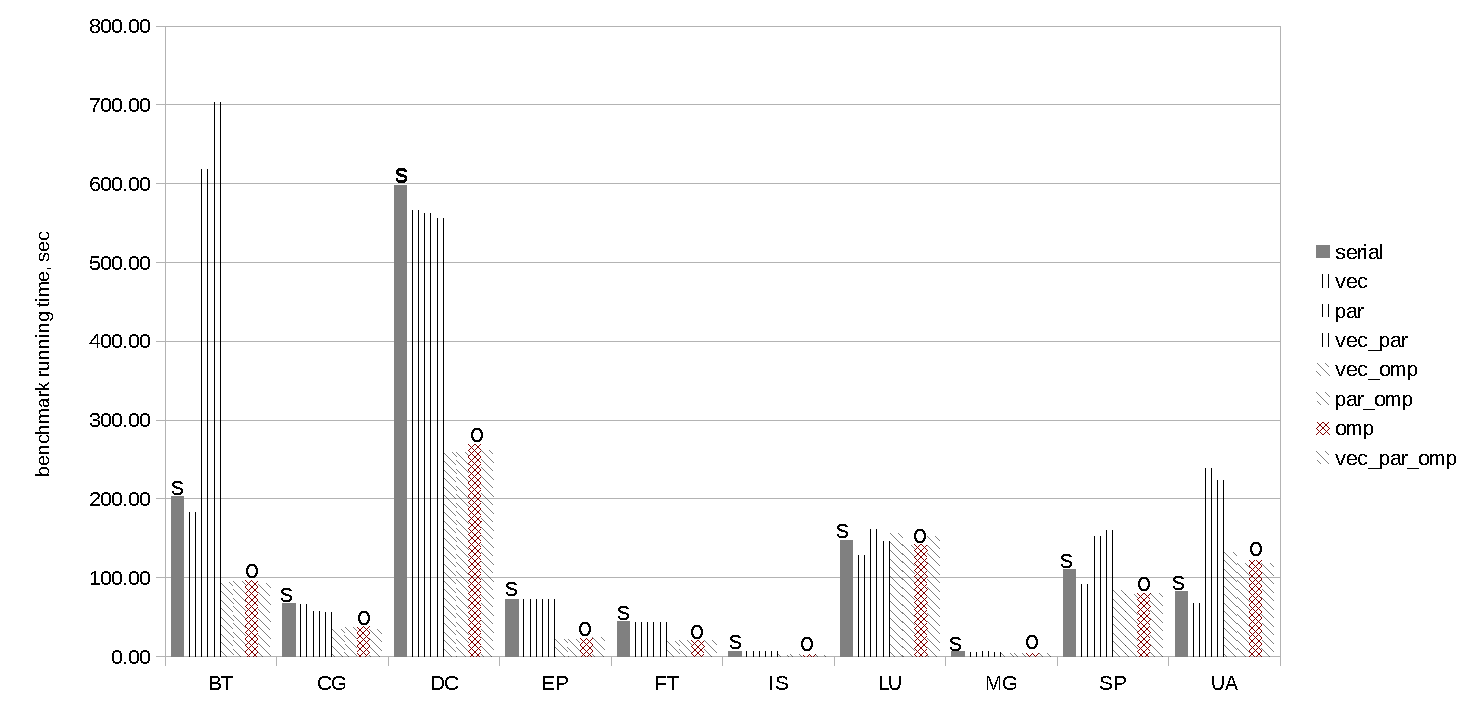
\includegraphics[width=1.0\textwidth]{images/benchmark_runtime.pdf}
\caption{The running time of various NPB benchmarks versions.}
\label{fig:benchmarks_runtime}
\end{figure}

\subsection{Limits of Machine Learning based methods}
\subsection{Data-Centric problem}
\quad As it has already been stated the problem of software parallelisation is multifaceted. There is a vast range of lower level technical issues, which can turn a perfectly parallelisable at a higher level computation into a non-parallelisable implementation. In our ML assistant project (see Chapter \ref{chapter_ml_assistant}) we showed that the main reasons of Intel Compiler failures on SNU NPB benchmarks are alias analysis conservativeness, uninlined function calls and statically unresolvable dependencies. The assistant tool we designed targets these aspects of the software parallelisation problem. But, there are many more reasons leading to non-parallelisable algorithm implementations. Source code listings \ref{lst:array} and \ref{lst:list} brightly illustrate yet another unsolved problem.\newline\null
\begin{minipage}[t]{0.45\linewidth}
\begin{lstlisting}[caption={Parallelisable loop operating on a \textbf{linear array}.},label={lst:array},language=C]
for (int i=0; i<n; it++) {
  a[i]=a[i]+1;
}
\end{lstlisting}
\end{minipage}
%
\begin{minipage}[t]{0.55\linewidth}
\begin{lstlisting}[caption={Non-parallelisable loop operating on a \textbf{linked-list}.},label={lst:list},language=C]
for (p=list; p!=NULL; p=p->next) {
  p->value+=1;
}
\end{lstlisting}
\end{minipage}
\quad Listings \ref{lst:array} and \ref{lst:list} illustrate two alternative implementations of the same simple computation. We increment all sequence elements by one. Listing \ref{lst:array} implements the sequence with a regular array linearly laid out in the memory. Listing \ref{lst:list} chooses a linked list as an implementing data structure, which leads to a source code non-parallelisability.\newline\null
\quad The DCP problem is not solved. Automatic methods are limited to relatively simple code bases such as libraries of well known data structures. The most successful methods rely on dynamic analysis and mamory graphs. Static techniques such as shape analysis are undecidable and highly conservative and might not finish in a reasonable time for the real software projects. Section [] gives a detailed literature review on the topic. 


\subsection{Parallel Programming Models}
\quad With a number of various hardware and operating system vendors entering the market with their different hardware architectures and system call interfaces software portability became a serious concern.   



To combat the problem industry vendors and major organisation came to design industry standards such as POSIX, OpenMP and MPI. 



\section{Data-Centric Parallelization}
\label{chapter_dcp}
\subsubsection{The Problem}
\quad As it has already been stated the problem of software parallelisation is multifaceted. There is a vast range of lower level technical issues, which can turn a perfectly parallelisable at a higher level computation into a non-parallelisable implementation. In our ML assistant project (see Chapter \ref{chapter_ml_assistant}) we showed that the main reasons of Intel Compiler failures on SNU NPB benchmarks are alias analysis conservativeness, uninlined function calls and statically unresolvable dependencies. The assistant tool we designed targets these aspects of the software parallelisation problem. But, there are many more reasons leading to non-parallelisable algorithm implementations. Source code listings \ref{lst:array} and \ref{lst:list} brightly illustrate yet another unsolved problem.\newline\null
\begin{minipage}[t]{0.45\linewidth}
\begin{lstlisting}[caption={Parallelisable loop operating on a \textbf{linear array}.},label={lst:array},language=C]
for (int i=0; i<n; it++) {
  a[i]=a[i]+1;
}
\end{lstlisting}
\end{minipage}
%
\begin{minipage}[t]{0.55\linewidth}
\begin{lstlisting}[caption={Non-parallelisable loop operating on a \textbf{linked-list}.},label={lst:list},language=C]
for (p=list; p!=NULL; p=p->next) {
  p->value+=1;
}
\end{lstlisting}
\end{minipage}
\quad Listings \ref{lst:array} and \ref{lst:list} illustrate two alternative implementations of the same simple computation. We increment all sequence elements by one. Listing \ref{lst:array} implements the sequence with a regular array linearly laid out in the memory. Listing \ref{lst:list} chooses a linked list as an implementing data structure, which leads to a source code non-parallelisability.\newline\null
\quad In the project of "Data-Centric Parallelisation (DCP)" we would like to automatically recognise 
\subsubsection{Literature Review}
\label{dcp_literature_review}
\quad The idea of automatic discovery of higher level entities in programs is not a new one. This discovery problem is closely interlinked and entangled with alias analysis techniques \cite{Muchnick:1998:ACD:286076} like points-to analysis \cite{Emami:1994:CIP:178243.178264}. Points-to analysis is a variation on data flow analysis techniques. The final output is the sets of pairs of the form (\textit{p},\textit{x}) (pointer variable \textit{p} points to a stack allocated variable \textit{x}). These techniques are aimed at getting aliasing information regarding stack-allocated pointers.\newline\null
\quad The problem of understanding heap-directed pointers and heap-allocated linked data structures these pointers might point to is addressed with a family of static analysis techniques collectively known as shape analysis. Shape analysis techniques can be used to verify properties of dynamically allocated data structures in compile time. These are among the oldest and most well known techniques. Three-valued logic \cite{Sagiv:1999:PSA:292540.292552}\cite{Wilhelm:2000:SA:647476.760384} can be used as an example. The technique proposes a construction of a mathematical model consisting of logical predicate expressions. The latter correspond to certain pointer operating imperative language program statements. Abstract interpretation of these statements leads to a construction of sets of shape graphs at various program points. Shape graphs approximate the possible states of heap-allocated linked data structures and answer the questions such as node reachability, data structure disjointness, cyclicity, etc. The major limitation of these simplified mathematical models is the lack of precision high level of abstraction leads to. The problem of precise shape analysis is provably undecidable.\newline\null
\quad The work of \cite{Ghiya:1996:TDC:237721.237724} proposes a simplified and hence more practical implementation of shape analysis. Authors propose to use direction \textit{D} and interference \textit{I} matrices instead of complex mathematical models in order to derive shape information on heap allocated data structures. The entry of direction matrix \textit{D[p,q]} says if there exists a path from a node referred to by \textit{p} to a node referred to by q. In other words, if we can enter a path withing the data structure through \textit{p} and exit through \textit{q}. The entry of interference matrix \textit{I[p,q]} says if the paths started from \textit{p} and \textit{q} are going to intersect at some point. Authors implement their technique withing McCAT compiler, which uses SIMPLE intermediate representation with a total of 8 statements (\textit{malloc()}, pointer assignments \textit{p=q}, structure updates \textit{p-$>$next=q}), which are capable of changing \textit{D} and \textit{I} matrices. Statements generate and kill entries in matrices. Moreover, they are capable of changing \textit{Shape} attribute of pointers. The technique has been assessed on various benchmarks (bintree, xref, chomp, assembler, loader, sparse, etc.) from the era before the standard benchmark suites became available. The technique mostly reported shapes as \textit{Trees} (be it a binary tree or a linked-list) or sometimes as \textit{DAGs} or \textit{Cycles} but with higher error rates in these last cases. The latter shows that the technique is imprecise and conservative.\newline\null
\quad One of the more recent techniques designed and developed by Philip Ginsbach and Michael F. P. O’Boyle is based on the pattern matching on LLVM IR level. The main idea is to specify computational idioms to be recognized in a domain specific constraint based programming language CAnDL \cite{Ginsbach:2018:CDS:3178372.3179515}. Constraints are specified over LLVM IR entities such as instructions, basic blocks, functions, etc. The CAnDL language allows for a rapid prototyping of new compiler optimisations based on pattern recognition and its substitution with an optimised versions of matched idioms. The language and its relatively fast backtracking constraint solver are capable of recognizing not only simple arithmetic idioms (thus performing different peephole optimizations), but more complex computations like general reductions and histograms \cite{Ginsbach:2017:DEG:3049832.3049862}, vector products in graphics shaders \cite{Ginsbach:2018:AML:3296957.3173182}, sparse and dense linear algebra computations and stencils \cite{Ginsbach:2018:AML:3296957.3173182}. Having recognized these computational idioms the work \cite{Ginsbach:2018:AML:3296957.3173182} replaces them with a code for various heterogeneous APIs (MKL, libSPMV, Halide, clBLAS, CLBlast, Lift) and compares the resulting performance demonstrating an improvement over sequential versions and matching performance to a hand-written parallel versions. The technique has been deployed on the sequential C versions of SNU NPB, the C versions of Parboil and the OpenMP C/C++ versions of Rodinia demonstrating an improved detection capabilities over the state-of-the-art techniques.\newline\null
\quad The other principally different technique has been recently proposed by Changhee Jung and Nathan Clark \cite{1669122}. The authors developed a Data-structure Detection Tool (DDT) based on LLVM framework. The tool instruments loads, stores and calls withing program binaries and gathers dynamic traces for sample inputs. The traces are used to recreate a memory allocation graph for program data structures. Call graphs are used to identify interface functions interacting with the built memory graph. DDT traces memory graph properties (number of nodes, edges, etc.) before and after interface function calls into another Daikon tool to compute dynamic invariants (the number of nodes in a memory graph decreses by 1 after every \textit(delete()) interface method call, etc.). At the end manually constructed decision tree is used to probabilistically match observed behavioral patterns against known data structure invariant properties. The technique has been deployed to recognise data structure implementations withing standard libraries like STL, Apache (STDCXX), Borland (STLport), GLib, Trimaran achieving almost perfect recognition accuracy. Moreover, the technique has been able to recognise linked lists in Em3d and Bh Olden benchmarks, along with red-black trees implementing vectors in Xalancbmk benchmark.\newline\null
\quad There has recently been other published works on the application of dynamic techniques to the problem of dynamic data structure recognition \cite{Rupprecht:2017:DID:3155562.3155607}\cite{Haller:2016:SDS:2938006.2938029}. The technique used in the DDT tool \cite{1669122} makes an assumption, that all modifications and interactions with memory graphs representing data structures happen through a set of interface functions. That is not true, when we deal with aggressively optimising compilers, which may eliminate some code or inline some functions. The MemPick tool \cite{Haller:2016:SDS:2938006.2938029} searches data structures directly on a built dynamic memory graph by analyzing its shape. The graph is built with the help of Intel Pin binary instrumentation tool during quiescent periods, when pointer operations are absent. DSIbin tool \cite{Rupprecht:2017:DID:3155562.3155607} operates with the source code rather than program binaries. Instead of memory points-to graphs it uses strands as primitives, which abstract such entities as singly-linked lists.\newline\null
\quad The work of Dekker \cite{Dekker:1994:ADS:3107859.3107876} addresses software design recovery problem in a completely different way. Contrary to the approaches described above, which operate on the IR and dynamic instruction stream levels, work of Dekker operates at the level of abstract syntax tree. Dekker's tool tries to compact the tree down to a recognizable syntactic patterns by transforming it in accordance to a special grammar.


\section{OOP and Software Design Patterns}
\quad Object-oriented software design is a complex topic in itself, which spawns a number of problems and questions. 

\quad Software design patterns are reusable solutions to common design problems in object-oriented software engineering. They live at the level higher than that of a source code and are language agnostic. The solutions can be regarded as standard solutions to design problems they target. These solutions have been well tested and proven to be the most reliable and elegant.

Chain of responsibility pattern is very similar to fold.
Visitor pattern roughly corresponds to fold.

\section{Imperative and Functional programming}
\quad Programming languages can be classified by different programming paradigms they support. Among the most general classifications are imperative and declarative programming paradigms.\newline\null
\quad Imperative programs are written in a form of instruction sequences, which read and write the state of a program. The concept of state is the main characteristic of imperative programming paradigm. Instruction sequences can be structured in various ways. In procedural programming paradigm instructions are grouped inside procedures and functions. In object-oriented programming (OOP) paradigm instructions are grouped with the data they operate on inside objects of various types or classes.\newline\null
\quad Declarative programs do not specify the exact sequence of steps and state updates a program needs to do in order to get the desired result. Declarative programs declare the properties of the desired result. The properties can be specified as a set of constraints like in constraint programming or a set of linear inequalities like in linear programming. Functional programming is another subtype of declarative programming. In functional programming the final desired result is specified as a sequence of stateless function evaluations. Among the most common functions are map, reduce, fold, etc.

\section{Parallel Algorithmic Skeletons}




